\chapter*{Shaders}

\section*{Purpose}
The purpose was to create an outline that indicates to users whether the object they are nearing is interactable. The important objects in the scenario are the laparoscopic tools, the robot arms, and other items such as scissors and scalpels. Somehow indicating that items can be interacted with is important in VR and in many other graphical environments such as games.

\section*{Method}
Two different outlines were created using different techniques; inverted normal meshes and post processing. Inverted normal meshes, or front face culling, are applied over the regular mesh and upscaled slightly. They are easy on GPUs compared to many post processing effects, but lack in customizability and accessibility during runtime. They also get increasingly visually disruptive when applied to detailed meshes. Post processing is usually computationally expensive compared to the previous method since they require at least an extra depth render, but they perform better in edge cases (such as overlapping), and are very customizable even during runtime. This was implemented using Unreal Engine's post processing stack, a custom depth render on important objects, and a global custom material. In the case of overlapping, for example when users grab the objects, inverted normal meshes work as any other mesh in that it renders to the depth buffer, whereas post-processing requires an extra check for depth at each position.

The post-processing effect was implemented using edge detection. This means that colour differences at edges are detected, and a linear interpolation from normal colours to a chosen outline colour decides which to render based on a parameter called edge angle falloff.

\section*{Results}

\begin{figure}[H]
\centering
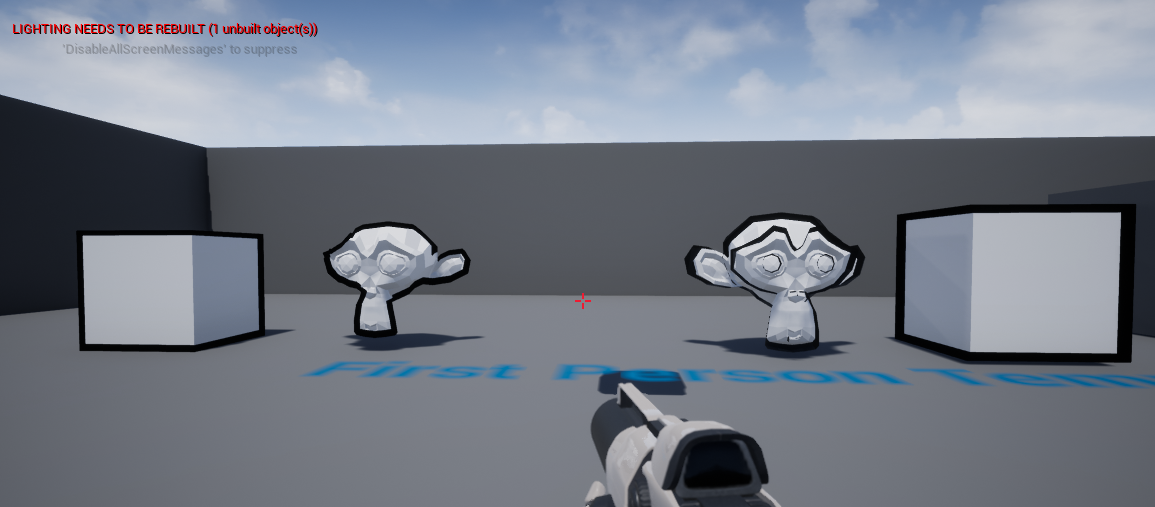
\includegraphics[width=1.0\textwidth]{Shader/comparison.png}
\caption{Comparison between methods. Left: Post processing, line width 3. Right: Inverted normals mesh, upscaled 1.1}
\label{fig:comparison}
\end{figure}

Figure \ref{fig:comparison} shows the two methods compared to each other. The inverted normal mesh is upscaled to 1.1 and uses black for both its main colour and its emission (meaning it is independent from light source blending). The post-processing effect uses texel width 3 and edge angle falloff -100 (which appears to only detect outer edges).

The post processing outline is a part of the mesh, whereas the inverted normals mesh extends over the regular mesh. The right side also shows some differences in line width, as well as some irregular lines around the eyes. On the left side, the lines being part of the monkey head mesh is also very obvious, as some of the detail is lost. 

\section*{Conclusion}

Based on these results, we implemented the post-processing effect on the interactable objects in the scene. These were easily accessible and customizable, and provided a consistent look on all objects and at all angles without creating new meshes. The problem with detail loss from the outlines extending into the mesh was not an issue since the effect only appeared once users were close enough to grab the objects.
